%%%%%%%%%%%%%%%%%%%%%%%%%%%%%%%%%%%%%%%%%%%%%%%%%%%%%%%%%%%%%%%%%%%%%%%%%%%%
\documentclass[a4j]{jarticle}

\usepackage{jsaisig}
% \usepackage{graphicx}
\usepackage[dvipdfmx]{graphicx}

%%%%%%%%%%%%%%%%%%%%%%%%%%%%%%%%%%%%%%%%%%%%%%%%%%%%%%%%%%%%%%%%%%%%%%%%%%%

\begin{document}

% 和文タイトル
\title{人工知能学会研究会 原稿フォーマットサンプル}

% 英文タイトル
\etitle{JSAI SIGs Conference Paper Format Sample}

% 著者名:
%	・各著者を\quad(全角空白)区切りで列挙
% 	・著者名の直後に\afil{所属番号}を追加→所属番号を上付で出力(\textsuperscript{所属番号}と同じ)
% 	 複数機関へ所属している場合は番号をカンマ区切りで列挙(下記著者2参照)
%  ・Corresponding Authorについては所属の後に\thanksを続け,連絡先を記入
%	・英文著者はカンマ区切りで列挙

\author{矢野 優雅\afil{1}%
	\thanks{連絡先:九州工業大学大学院生命体工学研究科人間知能システム工学専攻 \newline%
		      〒808-0135 福岡県北九州市若松区ひびきの2-4 \newline%
		      E-mail: yano.yuuga158@mail.kyutech.jp}\quad%
	福田 有輝也\afil{1}
	小野 智寛\afil{1}
	田向 権\afil{1,2}\\
	Yuga Yano\afil{1}\quad \quad Yukiya Fukuda\afil{1}\quad \quad Tomohiro Ono\afil{1}\quad \quad Hakaru Tamukoh\afil{1,2}}

% 所属
\affiliation{%
	\afil{1} 九州工業大学大学院生命体工学研究科\\
	\afil{1} Kyushu Institute of Technology Graduate School of Life Science and Systems Engineering\\
	\afil{2} 九州工業大学ニューロモルフィックAIハードウェア研究センター\\
	\afil{2} Research Center for Neuromorphic AI Hardware}

\abstract{
Abstract (English) comes here.......................................................
}

\maketitle
\thispagestyle{empty}

%%%%%%%%%%%%%%%%%%%%%%%%%%%%%%%%%%%%%%

\section{序論}
近年,少子高齢化の影響によってホームサービスロボットへの注目が集まっている.
また,ホームサービスロボットの発展を目的として,RoboCup@Homeが開催されている.
RoboCup@Homeは,実際の家庭環境を模した部屋でロボットを動作させ,様々なタスクに挑戦し得点を競う大会である.

%%%%%%%%%%%%%%%%%%%%%%%%%%%%%%%%%%%%%%

\section{提案方法}

□□□□□□□□□□□□□□□□□□□□
□□□□□□□□□□□□□□□□□□□□
□□□□□□□□□□□□□□□□□□□□
□□□□□□□□□□□□□□□□□□□□
...

\subsection{サブセクション}
□□□□□□□□□□□□□□□□□□□□
□□□□□□□□□□□□□□□□□□□□
%
\begin{figure}[ht]
  \centering
  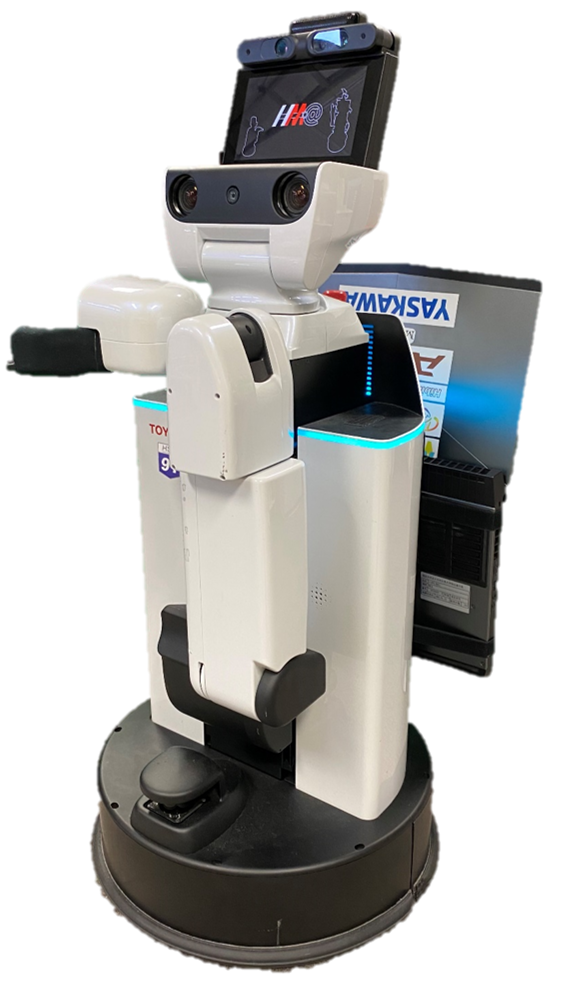
\includegraphics[width=2cm]{images/hsr_front.png}
  \caption{図の挿入例.}
  \label{fig:ex1}
\end{figure}
%
□□□□□□□□□□□□□□□□□□□□
□□□□□□□□□□□□□□□□□□□□
□□□□□□□□□□□□□□□□□□□□
□□□□□□□□□□□□□□□□□□□□
□□□□□□□□□□□□□□□□□□□□
%
\begin{table}[h]
  \centering
  \caption {表の挿入例.}
  \label{table:ex1}
  \begin{tabular}{c|cc}
    \hline
           & $a_1$ & $a_2$ \\ \hline
    $x_1$  &  0.1  &  0.1  \\
    $x_2$  &  0.2  &  0.2  \\ \hline
  \end{tabular}
\end{table}
%
□□□□□□□□□□□□□□□□□□□□
□□□□□□□□□□□□□□□□□□□□
....

図表の参照例:図\ref{fig:ex1},表\ref{fig:ex1}

参考文献の引用例:\cite{Sample1}\cite{Sample2}

%%%%%%%%%%%%%%%%%%%%%%%%%%%%%%%%%%%%%%

\section{むすび}
□□□□□□□□□□□□□□□□□□□□
□□□□□□□□□□□□□□□□□□□□
....

%%%%%%%%%%%%%%%%%%%%%%%%%%%%%%%%%%%%%%

\section*{謝辞}

□□□□□□□□□□□□□□□□□□□□
□□□□□□□□□□□□□□□□□□□□
....

%%%%%%%%%%%%%%%%%%%%%%%%%%%%%%%%%%%%%%

\begin{thebibliography}{99}
%\small

\bibitem{Sample1}
Author, A., Author, B.:
JSAI SIGs Conference Paper Format Sample,
{\it International Journal of Examples}, Vol.~19, No.~4, pp.~1--2 (2007)

\bibitem{Sample2}
第一著者, 第二著者:
人工知能学会研究会原稿フォーマットサンプル,
{\it International Journal of Examples}, Vol.~19, No.~4, pp.~1--2 (2007)

\end{thebibliography}

\end{document}
